%========== Document settings ==========
\documentclass[11pt,a4paper,twoside,openany]{report}
\setlength\textwidth{145mm}
\setlength\textheight{247mm}
\setlength\oddsidemargin{14.2mm}
\setlength\evensidemargin{0mm}
\setlength\topmargin{0mm}
\setlength\headsep{0mm}
\setlength\headheight{0mm}
\let\openright=\cleardoublepage

%========== Language settings ==========
\usepackage[main=british,czech]{babel}
\usepackage[utf8]{inputenc}
\usepackage[T1]{fontenc}

%========== Packages =============
\usepackage{stddoc}
\usepackage{circuitikz}

%========== Date format ===============
\newdateformat{monthyeardate}{\monthname[\THEMONTH] \THEYEAR}

%========== Declaration ==========
\newcommand\declarationpage{\clearpage
\vspace*{\fill}
\noindent\textbf{Declaration}\\[0.25cm]
I declare that I completed the presented thesis independently and that all used sources are quoted in accordance with the Methodological instructions that cover the ethical principles for writing an academic thesis.\\
\hrule\vspace*{1cm}

\noindent\textbf{Prohlášení}\\[0.25cm]
\foreignlanguage{czech}{Prohlašuji, že jsem předloženou práci vypracoval samostatně a že jsem uvedl veškeré použité informační zdroje v souladu s Metodickým pokynem o dodržování etických principů při přípravě vysokoškolských závěrečných prací.}\\
\begin{center}
	\begin{minipage}{0.45\textwidth}
		\begin{flushleft}
			V Praze, \hdashrule{3cm}{0.5pt}{2pt}
		\end{flushleft}
	\end{minipage}
	~
	\begin{minipage}{0.45\textwidth}
		\begin{flushright}
			\noindent\begin{tabular}{c}
				\\
				\hdashrule{4cm}{0.5pt}{2pt}\\
				Martin Šimák
			\end{tabular}
		\end{flushright}
	\end{minipage}
\end{center}
\clearpage}

%========== Acknowledgements ==========
\newcommand\acknowledgementspage{\clearpage
\vspace*{\fill}
\noindent\textbf{Acknowledgements}\\[0.25cm]
First and foremost, I would like to thank my supervisor, Jiří Velebil, for his outstanding guidance and his zeal throughout the creation of this thesis. Further, I would like to thank my family and my colleagues, namely Erik Rapp and Karolína Veselá, for their invaluable support.\\
\hrule\vspace*{1cm}

\noindent\textbf{Poděkování}\\[0.25cm]
\foreignlanguage{czech}{Především bych rád poděkoval svému vedoucímu, Jiřímu Velebilovi, za jeho vynikající vedení a za jeho zapálenost a vstřícnost během tvorby této práce. Dále bych rád poděkoval své rodině a svým kolegům, zejména Eriku Rappovi a Karolíně Veselé, za jejich neocenitelnou podporu.}
\clearpage}

%========== Abstract ==========
\newcommand\abstractpage{\clearpage
\noindent\textit{Title:}\\
\textbf{Connections on Differentiable Manifolds}\\[0.25cm]
\textit{Author:} Martin Šimák\\[0.25cm]
\textit{Study programme:} Open Electronic Systems\\[0.25cm]
\textit{Supervisor:} doc. RNDr. Jiří Velebil, Ph.D., Department of Mathematics FEE\\[0.25cm]
\textit{Abstract:}\\
One of the aims of this thesis is to fully introduce a comprehensive differentiable structure on a smooth manifold. To achieve that, we first inspect various aspects of its definition. Further, we introduce a tangent structure on said manifolds, allowing us to locally speak of derivatives and vector fields. This construction naturally results in definitions of a covariant derivative and a connection form, where the former serves as a generalization of a derivative in a direction and the latter as a tool for ``glueing'' tangent spaces together. As a climax of the thesis, we show that the two previously mentioned additional structures on the ambient manifold are equivalent.\\[0.25cm]
\textit{Keywords:} smooth manifolds, tangent structure, covariant derivative, connection\\[0.5cm]
\noindent\textit{Název práce:}\\
\textbf{Konexe na diferencovatelných varietách}\\[0.25cm]
\textit{Autor:} Martin Šimák\\[0.25cm]
\textit{Studijní program:} Otevřené elektronické systémy\\[0.25cm]
\textit{Vedoucí:} doc. RNDr. Jiří Velebil, Ph.D., katedra matematiky FEL\\[0.25cm]
\textit{Abstrakt:}\\
\foreignlanguage{czech}{Jedním z cílů této práce je v plném měřítku uvést rozsáhlou diferenciální strukturu na hladké varietě. Abychom toho dosáhli, prozkoumáme nejprve jednotlivé aspekty její definice. Dále na varietách uvedeme tečnou strukturu, jenž nám umožňuje lokálně hovořit o derivacích a vektorových polích. Tato konstrukce přirozeně vyúsťuje v definice kovariantní derivace a konexe, přičemž první z pojmů slouží jakožto zobecnění derivace ve směru a druhý jakožto nástroj pro \uv{slepování} tečných prostorů. Jako vyvrcholení práce ukážeme, že tyto dvě dodatečné struktury na varietě jsou ekvivalentní.}\\[0.25cm]
\textit{Klíčová slova:} hladké variety, tečná struktura, kovariantní derivace, konexe\\[0.5cm]
\clearpage}

%========== Bibliography ==========
\bibliographystyle{abbrvnat}

%========== Custom commands ==========
\newcommand{\Tx}{\mathrm{Tx}}
\newcommand{\Rx}{\mathrm{Rx}}

%========== Draft settings ==========
\usepackage{lipsum}


\makeindex
\begin{document}

    \pagenumbering{gobble}
    
    %========== Title page ==========
    % Suppress displaying the page number on the title page + count the following page as page 1 (not used)
    \begin{titlepage}
        % Define a new command for horizontal lines, change thickness here
\newcommand{\HRule}{\rule{\linewidth}{0.5mm}}
\center

%========== Header ==========
\textsc{\LARGE Czech Technical University in Prague,\\Faculty of Electrical Engineering}\\[1.5cm]
\textsc{\Large B2MPROJ6 - Thesis project}\\[0.5cm]
% \textsc{\Large Master's thesis}\\[0.5cm]

%========== Title ==========
\HRule\\[0.6cm]
{\huge\bfseries Inductive Wireless Power Transfer}\\[0.3cm] % Title of your document
\HRule\\[1.5cm]

%========== Authors ==========
\begin{minipage}{0.45\textwidth}
    \begin{flushleft}
        \large
        \textit{Author}\\
        M. \textsc{Šimák}\\
        \textsc{Department of Electromagnetic Field}
    \end{flushleft}
\end{minipage}
~
\begin{minipage}{0.45\textwidth}
    \begin{flushright}
        \large
        \textit{Supervisor}\\
        Ing. J. \textsc{Kraček}, Ph.D.\\
        \textsc{Department of Electromagnetic Field}
    \end{flushright}
\end{minipage}

%========== Logo ==========
% Position at 3/4 of the screen
\vfill\vfill\vfill

\includegraphics[width=0.3\textwidth]{src/ctu_logo_black.jpg}

%========== Date ==========
\vfill\vfill
{\large\monthyeardate\today}
% Push the date up 1/4 of the remaining page
\vfill
    \end{titlepage}

    %========== Blank page ==========
    \newpage\blankpage

    % %========== Assignment ==========
    % 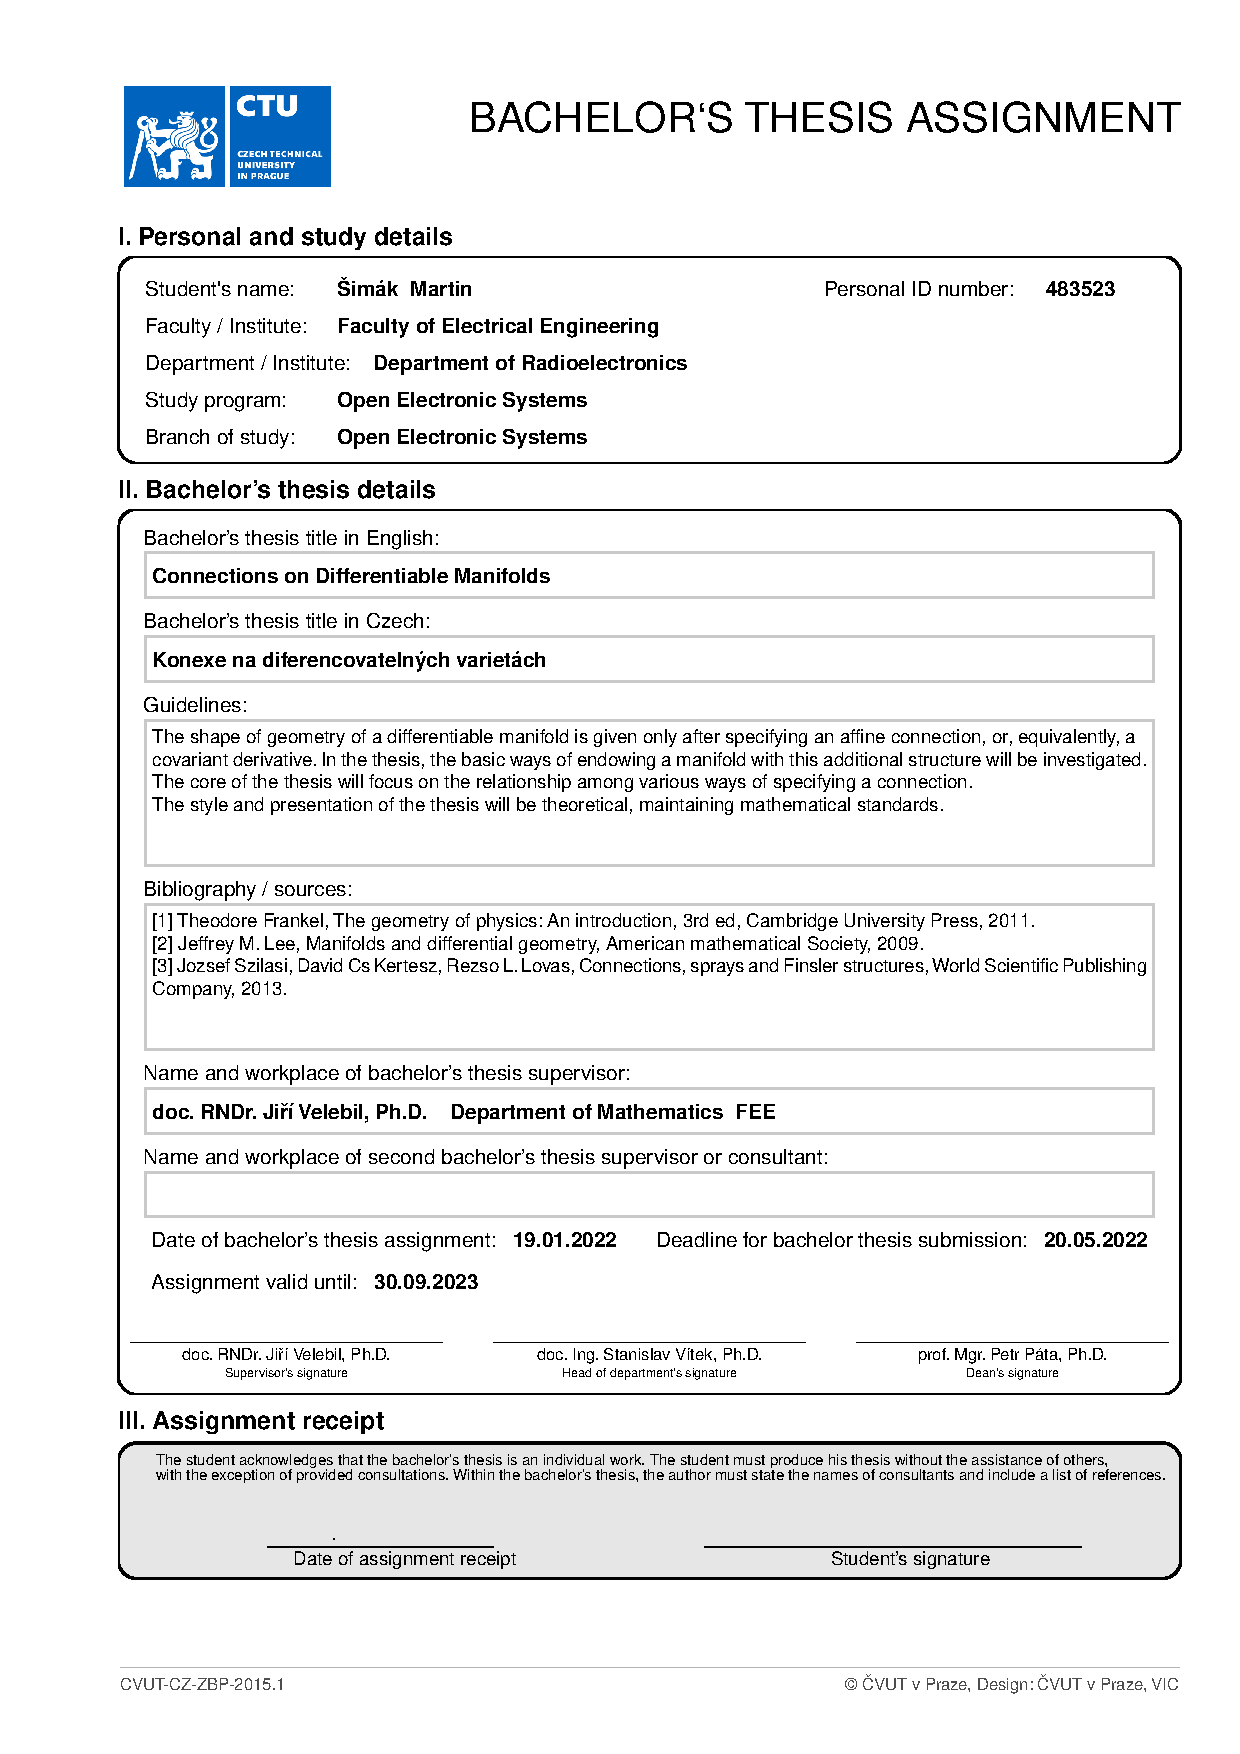
\includepdf[pages=-]{src/assignment.pdf}

    % %========== Blank page ==========
    % \newpage\blankpage

    % Start counting pages in roman numerals
    \pagenumbering{roman}

    % %========== Declaration ==========
    % \declarationpage

    % %========== Acknowledgements ==========
    % \acknowledgementspage

    % %========== Abstract ==========
    % \abstractpage

    % Start counting pages in arabic numerals
    \pagenumbering{arabic}

    %========== Table of contents ==========
    \tableofcontents

    %========== Introduction ==========
    % This is just a very vague introduction for the thesis project which is to be rewritten later on.
    \chapter*{Introduction}
    \label{chap:introduction}
    \addcontentsline{toc}{chapter}{\nameref{chap:introduction}}
    
    In recent years, the landscape of wireless power transfer (WPT) has undergone a significant transformation, fueled by the growing demand for convenient and efficient energy transfer methods in various industries. Among the plethora of wireless power transfer technologies, inductive wireless power transfer (IWPT) has emerged as a promising solution, particularly in the automotive sector. This project aims to delve into the fundamentals of inductive wireless power transfer, focusing on key aspects such as basic configuration, simulation of resistance and inductance, and a comparative analysis of simulation results against analytical formulae.

    The automotive industry is undergoing a paradigm shift towards electric vehicles (EVs) and the integration of advanced technologies. As vehicles become more electrified, the demand for efficient and seamless methods of charging electronic devices within the vehicle, such as mobile phones, has intensified. Inductive wireless power transfer, characterized by the transmission of energy through magnetic fields, has garnered attention for its potential to provide a convenient and cable-free charging experience. This project addresses the burgeoning need for a deeper understanding of IWPT systems and their design parameters.

    \paragraph*{Synopsis.} In \textbf{Chapter~\ref{chap:introduction-to-iwpt}}, we aim to explore the basic configuration of inductive wireless power transfer systems. This chapter also introduces the tools for analysis of IWPT systems, such as equivalent circuit models.

    \textbf{Chapter~\ref{chap:simulation-of-iwpt-systems}} conducts simulations of resistance and inductance using ANSYS Maxwell software, with a particular focus on zero frequency (DC) scenarios. Further on, we compare simulation results with analytical formulae to validate the accuracy and reliability of the simulation model.

    \paragraph*{Methodology.} The research methodology involves a step-by-step exploration of inductive wireless power transfer, starting with a theoretical foundation and progressing to detailed simulations using ANSYS Maxwell software. The comparison of simulation results with analytical formulae will provide a rigorous validation process.


    %========== Chapter 1: Introduction to inductive wireless power transfer ==========
    \chapter{Introduction to inductive wireless power transfer}
    \label{chap:introduction-to-iwpt}

    Wireless power transfer (WPT) in general is a mechanism which can be intermediated by the means of various technologies operating at different power levels and feasible distances. These technologies include far-field WPT which can be implemented by adopting an acoustic, optical or electromagnetic wave as the energy carrier. On the other hand, there are various near-field techniques utilizing the inductive coupling effects of non-radiative electromagnetic fields. The emphasis of this document is on the inductive variant due to its higher efficiency and thus industrial applicability.

    This chapter delves into the foundational aspects of IWPT systems. The primary objective is to elucidate the basic configurations employed in IWPT technology. Furthermore, this chapter introduces crucial analytical tools essential for understanding and optimizing IWPT systems, notably equivalent circuit models.

    \section{Equivalent circuit analysis}

        In general, a wireless power transmission chain from source to appliance can be rather complex and its in-depth investigations have been published, such as the power balance in~\cite{kracek-mazanek:power-balance-of-inductive-wireless-power-transfer}. The circuit model of the inductive transmission chain is depicted in Figure~\ref{fig:circuit-model-of-a-transmission-chain} along with the matching network on the side of the source and complex load representing the appliance energy sink.
        \begin{figure}[!ht]
            \centering
            \resizebox{\textwidth}{!}{%
            \begin{circuitikz}[american,>=Latex]
                % Parameters
                \def\ComponentLength{3}
                \def\ComponentHeight{.5}
                \def\CircuitXMargin{.5}
                \def\CircuitYMargin{.5}
                \def\SourceFCWidth{1}
                \def\InnerBlockHeight{2*\CircuitYMargin+\ComponentLength}
                \def\InnerBlockXMargin{.4}
                \def\InnerBlockYMargin{.7}
                \def\InnerBlockGap{.2}
                \def\OuterBlockGap{.7}

                % Source coordinates
                \coordinate (SourceCircuitBottomLeft) at (\InnerBlockXMargin+\SourceFCWidth+\InnerBlockGap+\CircuitXMargin,\InnerBlockYMargin+\CircuitYMargin) {};
                \coordinate (SourceCircuitBottomRight) at (\InnerBlockXMargin+\SourceFCWidth+2*\InnerBlockGap+3*\CircuitXMargin+2*\ComponentLength,\InnerBlockYMargin+\CircuitYMargin) {};
                \coordinate (SourceCircuitCentre) at (\InnerBlockXMargin+\SourceFCWidth+1.5*\InnerBlockGap+2*\CircuitXMargin+\ComponentLength,\InnerBlockYMargin+\CircuitYMargin+.5*\ComponentLength) {};
                \coordinate (MatchingNetworkBottomLeft) at ($(SourceCircuitBottomLeft)-(\CircuitXMargin,\CircuitYMargin)$) {};
                \coordinate (MatchingNetworkBottomRight) at ($(SourceCircuitCentre)-(.5*\InnerBlockGap,.5*\ComponentLength+\CircuitYMargin)$) {};
                \coordinate (SourceCouplingElementBottomLeft) at ($(SourceCircuitCentre)+(.5*\InnerBlockGap,-.5*\ComponentLength-\CircuitYMargin)$) {};
                \coordinate (SourceCouplingElementBottomRight) at ($(SourceCircuitBottomRight)+(\CircuitXMargin,-\CircuitYMargin)$) {};
                \coordinate (SourceBlockBottomLeft) at (0,0) {};
                \coordinate (SourceBlockBottomRight) at ($(SourceCouplingElementBottomRight)+(\InnerBlockXMargin,-\InnerBlockYMargin)$) {};
                % Appliance coordinates
                \coordinate (ApplianceCircuitBottomLeft) at ($(SourceCircuitBottomRight)+(2*\CircuitXMargin+2*\InnerBlockXMargin+\OuterBlockGap,0)$) {};
                \coordinate (ApplianceCircuitBottomRight) at ($(ApplianceCircuitBottomLeft)+(1.5*\ComponentLength+2*\CircuitXMargin+\InnerBlockGap,0)$) {};
                \coordinate (ApplianceCircuitCentre) at ($.5*(ApplianceCircuitBottomLeft)+.5*(ApplianceCircuitBottomRight)+(0,.5*\ComponentLength)$) {};
                \coordinate (ApplianceCouplingElementBottomLeft) at ($(ApplianceCircuitBottomLeft)-(\CircuitXMargin,\CircuitYMargin)$) {};
                \coordinate (ApplianceCouplingElementBottomRight) at ($(ApplianceCircuitCentre)-(.5*\InnerBlockGap,.5*\ComponentLength+\CircuitYMargin)$) {};
                \coordinate (ComplexLoadBottomLeft) at ($(ApplianceCircuitCentre)+(.5*\InnerBlockGap,-.5*\ComponentLength-\CircuitYMargin)$) {};
                \coordinate (ComplexLoadBottomRight) at ($(ApplianceCircuitBottomRight)+(\CircuitXMargin,-\CircuitYMargin)$) {};
                \coordinate (ApplianceBlockBottomLeft) at ($(ApplianceCouplingElementBottomLeft)-(\InnerBlockXMargin,\InnerBlockYMargin)$) {};
                \coordinate (ApplianceBlockBottomRight) at ($(ComplexLoadBottomRight)+(\InnerBlockXMargin,-\InnerBlockYMargin)$) {};

                % Source + FC block
                \draw (\InnerBlockXMargin,\InnerBlockYMargin) rectangle ++(\SourceFCWidth,\InnerBlockHeight);
                \node[anchor=center,rotate=90] at (\InnerBlockXMargin+.5*\SourceFCWidth,\InnerBlockYMargin+\CircuitYMargin+.5*\ComponentLength) {Source + FC};
                \draw[dashed] (\InnerBlockXMargin+\SourceFCWidth+.5*\InnerBlockGap,0) -- ++(0,2*\InnerBlockYMargin+\InnerBlockHeight);
                \draw[->] (\InnerBlockXMargin+.5*\SourceFCWidth,1.5*\InnerBlockYMargin+\InnerBlockHeight) -- ++(.5*\SourceFCWidth+.5*\InnerBlockGap,0) node[at start, left] {$P_{\mathrm{T}}$};
                % Source circuit
                \draw ($(SourceCircuitBottomLeft)-(\InnerBlockGap+\CircuitXMargin,0)$)
                    to[short, -*] ++(\InnerBlockGap+\CircuitXMargin,0)
                    to[short] ++(\ComponentLength+\CircuitXMargin+\InnerBlockGap+\CircuitXMargin+\ComponentLength,0)
                    to[L, l^=$L_{\mathrm{S}}$, mirror] ++(0,\ComponentLength)
                    to[generic, l^=$R_{\mathrm{S}}$] ++(-\ComponentLength,0)
                    to[short] ++(-2*\CircuitXMargin-\InnerBlockGap,0)
                    to[generic, l^=$X_{\mathrm{M}}$] ++(-\ComponentLength,0)
                    to[short, *-] ++(-\CircuitXMargin-\InnerBlockGap,0);
                \draw (SourceCircuitBottomRight)+(.5*\ComponentHeight,.2*\ComponentLength) node (SourceCouplingDot) {$\bullet$};
                % Source voltage arrow
                \draw[<-] (SourceCircuitBottomLeft) -- ++(0,.95*\ComponentLength) node[midway, right] {$U_{\mathrm{S}}$};
                % Loop current arrow
                \draw[->] ($(SourceCircuitCentre)+({2*cos(120)},{1*sin(120)})$) arc[start angle=120, delta angle=-330, x radius = 2, y radius = 1];
                \draw ($(SourceCircuitCentre)+(-1.5,0)$) node {$I_{\mathrm{S}}$};
                % Active power lost
                \draw[->] ($(SourceCircuitBottomRight)+(-.5*\ComponentLength,\ComponentLength+.5*\ComponentHeight)$) -- ++(-.5*\ComponentHeight+\CircuitYMargin+.5*\InnerBlockYMargin,-.5*\ComponentHeight+\CircuitYMargin+.5*\InnerBlockYMargin) node[at end, right] {$P_{\mathrm{S}}$};
                % Matching network block
                \draw (MatchingNetworkBottomLeft) rectangle ($(MatchingNetworkBottomRight)+(0,\InnerBlockHeight)$);
                \node[below] at ($.5*(MatchingNetworkBottomLeft)+.5*($(MatchingNetworkBottomRight)$)$) {Matching network};
                % Coupling element block
                \draw (SourceCouplingElementBottomLeft) rectangle ($(SourceCouplingElementBottomRight)+(0,\InnerBlockHeight)$);
                \node[below] at ($.5*(SourceCouplingElementBottomLeft)+.5*(SourceCouplingElementBottomRight)$) {Coupling Element};
                % Side of source block
                \draw (SourceBlockBottomLeft) rectangle ($(SourceBlockBottomRight)+(0,2*\InnerBlockYMargin+\InnerBlockHeight)$);
                \node[below] at ($.5*(SourceBlockBottomLeft)+.5*(SourceBlockBottomRight)$) {Side of source};

                % Appliance circuit
                \draw (ApplianceCircuitBottomLeft)
                    to[short] ++(1.5*\ComponentLength+2*\CircuitXMargin+\InnerBlockGap,0)
                    to[generic, l^=$Z_{\mathrm{L}}$] ++(0,\ComponentLength)
                    to[short] ++(-2*\CircuitXMargin-.5*\ComponentLength-\InnerBlockGap,0)
                    to[generic, l^=$R_{\mathrm{A}}$] ++(-\ComponentLength,0)
                    to[L, l^=$L_{\mathrm{A}}$, mirror] ++(0,-\ComponentLength) -- cycle;
                \draw (ApplianceCircuitBottomLeft)+(-.5*\ComponentHeight,.2*\ComponentLength) node (ApplianceCouplingDot) {$\bullet$};
                % Loop current arrow
                \draw[<-] ($(ApplianceCircuitCentre)+({1.6*cos(120)},{.8*sin(120)})$) arc[start angle=120, delta angle=-330, x radius = 1.6, y radius = .8];
                \draw ($(ApplianceCircuitCentre)+(-1.1,0)$) node {$I_{\mathrm{S}}$};
                % Active power lost
                \draw[->] ($(ApplianceCircuitBottomRight)+(-2*\CircuitXMargin-.5*\ComponentLength-\InnerBlockGap-.5*\ComponentLength,\ComponentLength+.5*\ComponentHeight)$) -- ++(-.5*\ComponentHeight+\CircuitYMargin+.5*\InnerBlockYMargin,-.5*\ComponentHeight+\CircuitYMargin+.5*\InnerBlockYMargin) node[at end, right] {$P_{\mathrm{A}}$};
                % Coupling element block
                \draw (ApplianceCouplingElementBottomLeft) rectangle ($(ApplianceCouplingElementBottomRight)+(0,\InnerBlockHeight)$);
                \node[below] at ($.5*(ApplianceCouplingElementBottomLeft)+.5*(ApplianceCouplingElementBottomRight)$) {Coupling Element};
                % Complex load block
                \draw (ComplexLoadBottomLeft) rectangle ($(ComplexLoadBottomRight)+(0,\InnerBlockHeight)$);
                \node[below] at ($.5*(ComplexLoadBottomLeft)+.5*(ComplexLoadBottomRight)$) {Complex Load};
                % Side of appliance
                \draw (ApplianceBlockBottomLeft) rectangle ($(ApplianceBlockBottomRight)+(0,2*\InnerBlockYMargin+\InnerBlockHeight)$);
                \node[below] at ($.5*(ApplianceBlockBottomLeft)+.5*(ApplianceBlockBottomRight)$) {Side of appliance};

                % Mutual coupling arrow
                \draw[<->, rounded corners=5mm] (SourceCouplingDot) to ($.5*(SourceCouplingDot)+.5*(ApplianceCouplingDot)+(0,.5)$) to (ApplianceCouplingDot);
                \node[anchor=south] at ($.5*(SourceCouplingDot)+.5*(ApplianceCouplingDot)+(0,.5)$) {$\kappa_{\mathrm{M}}$};
            \end{circuitikz}%
            }
            \caption{\label{fig:circuit-model-of-a-transmission-chain}Circuit model of a transmission chain}
        \end{figure}

        The mutually coupled inductors in the centre of Figure~\ref{fig:circuit-model-of-a-transmission-chain} can be redrawn using an equivalent circuit model as depicted in Figure~\ref{fig:mutually-coupled-inductors-equivalent-circuit}. Here, the coupling coefficient between the transmitting and receiving coils $\kappa_{\mathrm{M}}$ is represented by the mutual inductance:
        \begin{align}
            \kappa_{\mathrm{M}} &= \frac{M}{\sqrt{L_{\mathrm{S}}L_{\mathrm{A}}}}.
        \end{align}
        \begin{figure}[!ht]
            \centering
            \begin{circuitikz}[american, >=Latex]
                % Parameters
                \def\ComponentLength{3}
                \def\ComponentHeight{.5}

                \draw (0,0)
                    to[short, o-] ++(\ComponentLength,0)
                    to[L, l_=$M$] ++(0,\ComponentLength)
                    to[L, l_=$L_{\mathrm{S}}-M$, mirror] ++(-\ComponentLength,0)
                    to[short, -o] ++(0,0);
                \draw (\ComponentLength,0)
                    to[short, -o] ++(\ComponentLength,0);
                \draw (\ComponentLength,\ComponentLength)
                    to[L, l^=$L_{\mathrm{A}}-M$] ++(\ComponentLength,0)
                    to[short, -o] ++(0,0);

                \draw[<-] (0,.05*\ComponentLength) -- ++(0,.9*\ComponentLength) node[midway, right] {$U_1$};
                \draw[<-] (2*\ComponentLength,.05*\ComponentLength) -- ++(0,.9*\ComponentLength) node[midway, right] {$U_2$};
            \end{circuitikz}
            \caption{\label{fig:mutually-coupled-inductors-equivalent-circuit}Mutually coupled inductors -- equivalent circuit}
        \end{figure}
        
        Understanding inductive coupling in IWPT systems is paramount due to its pivotal role in enabling efficient energy transfer between coils. As depicted in Figure~\ref{fig:circuit-model-of-a-transmission-chain}, the mutual electromagnetic induction between the transmitter and receiver coils forms the core mechanism of IWPT. This coupling phenomenon determines the efficiency and reliability of power transfer, making it imperative for thorough investigation.

        Furthermore, Figure~\ref{fig:circuit-model-of-a-transmission-chain} highlights the significance of equivalent circuit analysis in comprehending inductive coupling. By abstracting the intricate interactions between coils into simplified models, equivalent circuits, such as the model in Figure~\ref{fig:mutually-coupled-inductors-equivalent-circuit}, provide a systematic framework for analyzing IWPT systems. Parameters such as impedance matching, resonance frequency, and power transfer efficiency, depicted in the equivalent circuit representation, offer crucial insights into system performance.

        In the following chapter, we perform a 3D CAD simulation applied to the basic configuration of coupled inductors, providing an approach for determining the values of resistances and inductances crucial to Figure~\ref{fig:circuit-model-of-a-transmission-chain}.

    %========== Chapter 2: Simulation of IWPT systems ==========
    \chapter{Simulation of IWPT systems}
    \label{chap:simulation-of-iwpt-systems}

    In this chapter, we delve into the simulation aspects of IWPT systems using \emph{Maxwell ANSYS} software. The focus of this investigation is on the simulation of basic coupled inductors, serving as a fundamental model for IWPT systems. Through these simulations, we aim to extract key parameters such as self and mutual inductance, as well as the DC resistance of both the transmitting and receiving coils.

    One of the primary objectives of this simulation study is to validate the accuracy of the simulated parameters against analytical formulae. By comparing the simulated values of self and mutual inductance, as well as DC resistance, with their analytically derived counterparts, we aim to assess the fidelity of the simulation model and its ability to capture the behavior of IWPT systems.

    \section{Simulation results}

        The simulation process involves setting up the geometries and material properties of the coils within the software environment, accurately representing the physical characteristics of the inductive components. By applying appropriate boundary conditions and excitation sources, we replicate the operational conditions of IWPT systems to obtain realistic results.

        For the validation of simulation results, we can construct a 3D CAD model of the basic IWPT configuration: coupled inductors. This model can be seen in Figure~\ref{fig:basic-coupled-inductors} with terminals reaching outside the figure to the edge of the simulation space. The bounding box dimensions must always be chosen great enough to encompass the vast majority of the excited field in order to minimize the numerical error caused by cutting off the simulation space. For the excitation of $\qty{1}{\A}$ applied to the terminals, a bounding cube with an edge of $\qty{200}{\mm}$ is sufficient for practical compliance with reality.
        \begin{figure}[!ht]
            \centering
            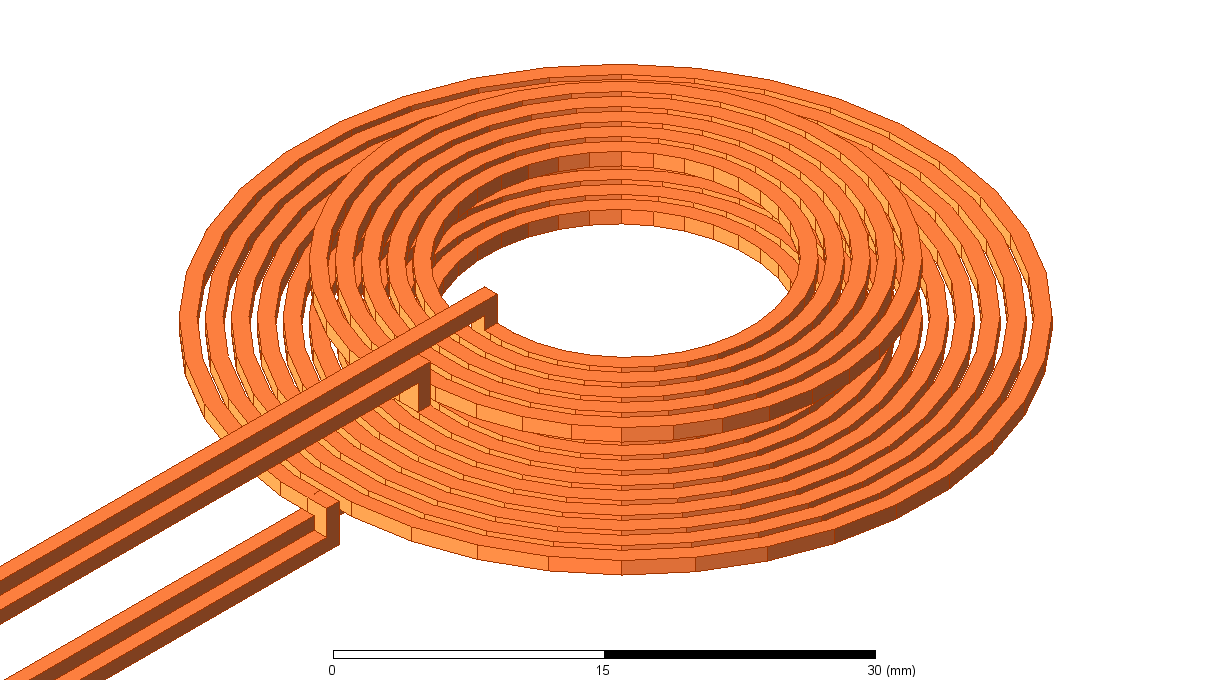
\includegraphics[width=.9\textwidth]{src/basic-coupled-inductors-isometric.png}
            \caption{\label{fig:basic-coupled-inductors}Basic coupled inductors}
        \end{figure}

        Performing analysis of the 3D CAD model in \emph{Maxwell ANSYS}, we can extract the values of resistance along with self and mutual inductance.%
            \footnote{The inductance values can be computed for DC excitation in the \emph{Magnetostatic solver} or for an arbitrary number of frequency points using the \emph{EddyCurrent solver}. These two solvers were found to yield identical results in the DC case.}
        In more detail, the simulation results of the DC resistance are
        \begin{align}
            \label{eq:dc-parameters-resistance-simulation}
            R_{\Tx} &= \qty{21.7}{\mohm},
        &
            R_{\Rx} &= \qty{10.5}{\mohm}.
        \end{align}
        Furthermore, the simulated DC inductance values are
        \begin{align}
        \label{eq:dc-parameters-inductance-simulation}
            L_{\Tx} &= \qty{3.8}{\uH},
        &
            L_{\Rx} &= \qty{1.0}{\uH},
        &
            M &= \qty{0.6}{\uH}.
        \end{align}

    \section{Analytical results}

        In this section, we aim to validate the simulation results using analytical formulae. Therefore, let us assume geometry identical to the 3D CAD model depicted in Figure~\ref{fig:basic-coupled-inductors}. This model features two inductors made of annealed copper, both with the same initial radius $\qty{10}{\mm}$ and linear radius change of $\qty{1.46}{\mm}$ per turn, and differring only in the number of turns. The transmitting coil has got $N_{\Tx} = 10$ turns, whereas the receiving coil has got only $N_{\Rx} = 5$ turns.

        \subsection{Resistance}

            The DC resistance $R$ of a wire of uniform cross-sectional area $A$, length $\l$ and resistivity $\rho$, can be calculated using the renowned formula
            \begin{align}
                \label{eq:dc-resistance-of-a-wire}
                R &= \frac{\rho \l}{A} = \frac{\l}{\sigma A},
            \end{align}
            where $\sigma$ is conductivity, the reciprocal of resistivity. Thus, in order to calculate this value, we need to find the lengths of the wires constituting the respective coils. Since we already know their spiral geometry parameters, we can write their corresponding formulas using the spiral equation
            \begin{align}
                \label{eq:spiral-equation}
                r(\theta) &= 10+\frac{1.46}{2\pi} \theta, \quad 0 \leq \theta \leq N\cdot 2 \pi,
            \end{align}
            where $N$ is the number of turns of the individual spiral. Following this, we can recall the theorem from real analysis for calculating the arc length of a graph in a polar coordinate system which goes as follows:
            \begin{theorem}
                \label{theorem:length-of-a-graph}
                Let $f$ be a real function of class~$C^1$ on $\(\alpha, \beta\)$, where $\alpha < \beta$. The arc length of the graph of $r=f(\theta)$ from $\theta=\alpha$ to $\theta=\beta$ is
                \begin{align}
                    \label{eq:length-of-a-graph}
                    \l &= \int_\alpha^\beta \sqrt{|f(\theta)|^2 + |f'(\theta)|^2} \,\d\theta = \int_\alpha^\beta \sqrt{r^2 + \(\frac{\partial r}{\partial \theta}\)^2} \,\d\theta.
                \end{align}
            \end{theorem}
            
            Substituting $N = 10$ for the transmitting coil and $N = 5$ for the receiving coil into Equation~\ref{eq:spiral-equation}, we obtain the spiral equations
            \begin{align}
                \label{eq:tx-spiral-equation}
                r_{\Tx}(\theta) &= 10+\frac{1.46}{2\pi} \theta, \quad 0 \leq \theta \leq 10\cdot 2 \pi
            \end{align}
            and
            \begin{align}
                r_{\Rx}(\theta) &= 10+\frac{1.46}{2\pi} \theta, \quad 0 \leq \theta \leq 5\cdot 2 \pi,
            \end{align}
            Furthermore, applying Theorem~\ref{theorem:length-of-a-graph}, we can calculate the lengths of the spirals as
            \begin{align}
                \l_{\mathrm{TxS}} &= \int_0^{10 \cdot 2\pi} \sqrt{\(10+\frac{1.46}{2\pi} \theta\)^2+\(\frac{1.46}{2\pi}\)^2} \,\d\theta \,\unit{\mm} \approx \qty{1087.1}{\mm},
            \\
                \l_{\mathrm{RxS}} &= \int_0^{5 \cdot 2\pi} \sqrt{\(10+\frac{1.46}{2\pi} \theta\)^2+\(\frac{1.46}{2\pi}\)^2} \,\d\theta \,\unit{\mm} \approx \qty{428.9}{\mm}.
            \end{align}
            For the total length of a coil, the feeding terminals must be taken into account:
            \begin{align}
                \l_{\mathrm{TxT1}} &= \qty{94.0}{\mm},
            &
                \l_{\mathrm{RxT1}} &= \qty{94.0}{\mm},
            \\
                \l_{\mathrm{TxT2}} &= \qty{86.7}{\mm},
            &
                \l_{\mathrm{RxT2}} &= \qty{79.5}{\mm}.
            \end{align}
            Hence, the final length of the transmitting and receiving coils are
            \begin{align}
                \label{eq:tx-length}
                \l_{\Tx} &= \l_{\mathrm{TxS}} + \l_{\mathrm{TxT1}} + \l_{\mathrm{TxT2}} = \qty{1267.8}{\mm},
            \\
                \label{eq:rx-length}
                \l_{\Rx} &= \l_{\mathrm{RxS}} + \l_{\mathrm{RxT1}} + \l_{\mathrm{RxT2}} = \qty{602.4}{\mm}.
            \end{align}

            At last, we can apply Equation~\ref{eq:dc-resistance-of-a-wire} to our case of the IWPT coils which consist of copper wire of cross-sectional area $A = \qty{1}{\mm\squared}$. The conductivity of annealed copper is $\sigma = \qty{5.8001e7}{\siemens\per\metre}$. With lengths given by Equations~\ref{eq:tx-length}~and~\ref{eq:rx-length}, we obtain the values of DC resistance
            \begin{align}
                \label{eq:dc-parameters-resistance-analytical}
                R_{\Tx} &= \qty{21.9}{\mohm},
            &
                R_{\Rx} &= \qty{10.4}{\mohm}.
            \end{align}

            Comparing these values with the simulation results contained in Equation~\ref{eq:dc-parameters-resistance-simulation}, we can confirm the accuracy of the simulation to $\approx\qty{0.2}{\mohm}$.
        
        \subsection{Inductance}
            
            The values of DC inductances, both self and mutual, are subject to complex computations using elliptic integrals. Luckily, we can utilize the astounding work~\cite{pankrac:power-inductors-part-3} which provides us with an elaborate guide on how to determine the self and mutual inductance of coaxial coils in air. Furthermore, the aforementioned work was supplemented with numerical software~\cite{pankrac-software:self-and-mutual-inductance-calculation-of-coaxial-coils-in-air} which performs all the complex calculations in response to simple input. This input is the task geometry:
            \begin{center}
                \begin{minipage}{.45\textwidth}
                    \paragraph{Transmitting coil:} \begin{itemize}
                        \item inner diameter: $\qty{20}{\mm}$,
                        \item outer diameter: $\qty{51}{\mm}$,
                        \item coil height: $\qty{1}{\mm}$,
                        \item number of turns: $\qty{10}{}$.
                    \end{itemize}
                \end{minipage}
                ~
                \begin{minipage}{.45\textwidth}
                    \paragraph{Receiving coil:} \begin{itemize}
                        \item inner diameter: $\qty{20}{\mm}$,
                        \item outer diameter: $\qty{36}{\mm}$,
                        \item coil height: $\qty{1}{\mm}$,
                        \item number of turns: $\qty{5}{}$.
                    \end{itemize}
                \end{minipage}
            \end{center}
            The axial coil distance is $\qty{10}{\mm}$. Using the fifth Romberg extrapolation $R(n,5)$ for estimation of the elliptic integrals, we obtain the values of inductance
            \begin{align}
                \label{eq:dc-parameters-inductance-analytical}
                L_{\Tx} &= \qty{3.8}{\uH},
            &
                L_{\Rx} &= \qty{0.9}{\uH},
            &
                M &= \qty{0.6}{\uH}.
            \end{align}

            Again, comparing these values with the simulation results in Equation~\ref{eq:dc-parameters-inductance-simulation}, we can confirm the accuracy of the simulation to $\approx\qty{0.1}{\uH}$.

    
    %========== Conclusion ==========
    \chapter*{Conclusion}
    \label{chap:conclusion}
    \addcontentsline{toc}{chapter}{\nameref{chap:conclusion}}
    
    In summary, this thesis project has effectively demonstrated the capabilities of Maxwell ANSYS software in simulating and analyzing Inductive Wireless Power Transfer (IWPT) systems. Beginning with an introductory overview of IWPT systems and equivalent circuit models in Chapter~\ref{chap:introduction-to-iwpt}, followed by a detailed simulation of basic coupled inductors in Chapter~\ref{chap:simulation-of-iwpt-systems}, we have established the software's reliability in capturing the electromagnetic behavior of such systems. The satisfactory agreement between simulated results and analytical formulas reaffirms the accuracy and robustness of Maxwell ANSYS, particularly in modeling IWPT systems with frequency dependencies and complex structures. These findings highlight the software's potential for designing and optimizing wireless power transfer technologies for practical applications. As we continue to refine simulation techniques and explore more sophisticated system configurations, the insights gained from this project will serve as a valuable foundation for future developments in the field.

    %========== Bibliography ==========
    \bibliography{bibliography}
	
    % %========== Index ==========
	% \printindex

\end{document}
